\section{TDN -- Design}\label{sec:design}

\comment{This section will cover the design of the SW, as specified through the requirements engineering document. Only the parts related to learning will be covered.}


As indicated in description of work (DOW) document, the objective of the AMIDST project is to provide an open source toolbox implementing novel developments in scalable algorithms for inference and learning with probabilistic graphical models able to operate in hybrid domains. 

The initial developed structure of AMIDST toolbox includes eight packages as shown in Figure \ref{Figure:ToolboxStructure}.

\begin{figure}[ht!]
\begin{center}
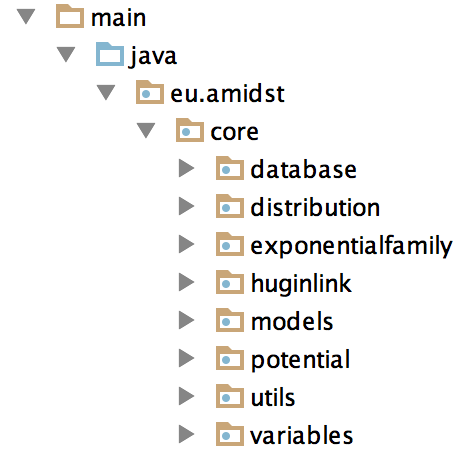
\includegraphics[scale=0.85]{./figures/ToolboxStructure} 
\caption{\label{Figure:ToolboxStructure} The main packages defined for Amidst toolbox.}
\end{center}
\end{figure}